% !TEX root =  ../master.tex
\chapter{Konzeption}
\section{Frontendarchitektur}
\section{Datenmodell und Datenhaltung}

Die Anwendung folgt dem \ac{MVC}-Pattern. Das heißt, die Anwendung ist aufgeteilt in 3 Bereiche:
\begin{itemize}%TODO: Hier kann man noch mehr schreiben
    \item Model\\
        Das Modell stellt den aktuellen Status bzw. den aktuellen Zustand der Anwendung dar.
    \item View\\
        Die Präsentation ist zuständig für die Darstellung der Daten und ermöglicht dem Benutzer die Interaktion mit diesen sowie die Steuerung der Anwendung.
    \item Controller\\
        Der Controller kümmert sich um die Steuerung der Anwendung. Er verwaltet die Präsentation und steuert den Datenfluss zwischen der Präsentation und dem Modell.
\end{itemize}
% \begin{wrapfigure}{r}{5.5cm}
%     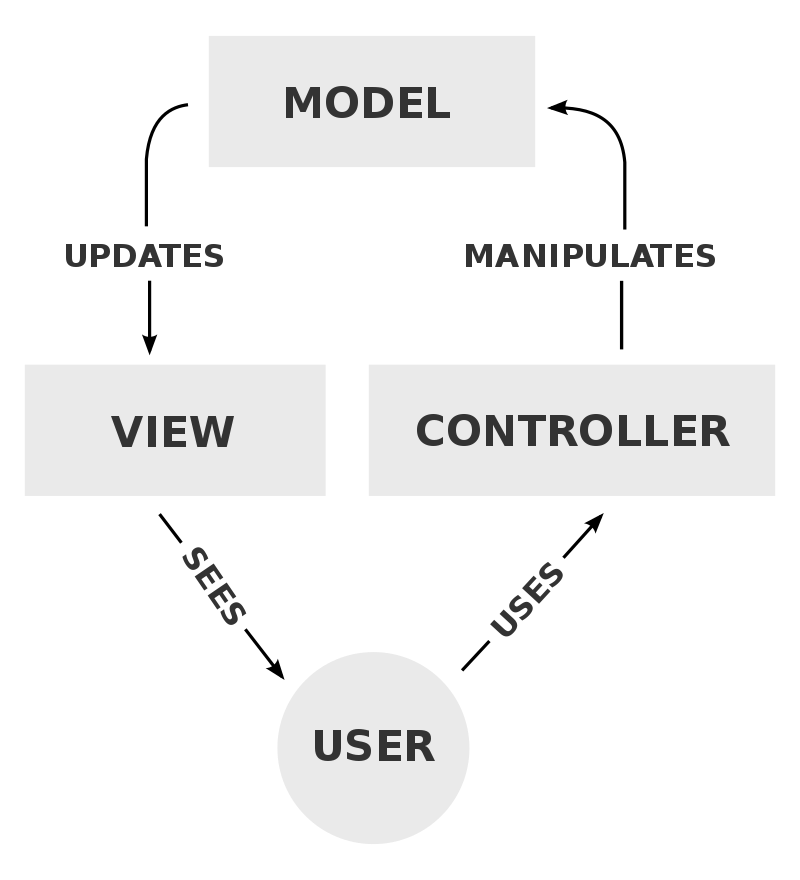
\includegraphics[width=.25\textwidth]{img/1024px-ModelViewControllerDiagram2.svg.png}
%     \caption{}
%     %TODO: https://en.wikipedia.org/wiki/Model%E2%80%93view%E2%80%93controller#/media/File:MVC-Process.svg
%   \end{wrapfigure} 

% TODO ER-Modell



\subsection{Studierende}
\subsection{Dozierende}
\subsection{Kurs erstellen}
\subsection{Karteikarten-Lernsystem}
\subsection{ToDo-Liste}
\section{Datensicherheit}
\section{Datenschutz}
\section{Grundlage für Datenauswertung}
% Hier Verweise auf Aubau und Bezug zum leichten Ausbau, etc.








\section{Ich mach hier einen WIP Abschnitt :D}
Aus den Anforderungen geht hervor, dass es zwei Nutzerrollen gibt: Dozenten und Studenten.
Dozenten sollen in der Anwendung ihre Kurse verwalten können.
Ein Kurs orientiert sich dabei an der Organisation, die in der Realität vorliegen.
Auch in vorhandenen Tools wie beispielsweise \enquote{Moodle} sind Studenten anhand von Kursen organisiert.
Aufgrund der Vielzahl an solchen Lösungen scheint sich eine solche Organisation zu bewähren.
Aus diesem Grund liegt es nahe, das auch die zu entwickelnde Anwendung eine solche Struktur nutzen sollte.
% TODO: Wie Werden Kurse erstellt

Nachdem nun geklärt wurde, wie die Organisation von Studenten und Dozenten stattfindet, muss nun die Zuweisung von Studenten zu Kursen die Zuweisung von Dozenten konzipiert werden.
Zunächst wird die Studentenzuweisung betrachtet.
Für die Zuweisung von Studenten kommen mehrere Ansätze in betracht, die sich in der Person unterscheiden, die die Zuweisung durchfüht :
\begin{enumerate}
    \item Zuweisung durch Anwendungsadministrator
    \item Zuweisung durch Dozenten
    \item Zuweisung durch Studenten
\end{enumerate}
Als erster Ansatz kommt die Zuweisung durch einen Anwendungsadministrator in betracht.
Ein solcher Administrator ist ein zentraler Mitarbeiter der DHBW, welcher komplette Autorität über die Anwendung besitzt.
Von einem solchen Ansatz wird abgesehen, da der Verwaltungsaufwand sehr hoch ausfällt.
Für jeden Kurs über 20 Studenten zuzuweisen, und das für mehrere Kurse pro Semester und Vorlesung, scheint nicht realistisch.

Der zweite ist der Ansatz der Zuweisung durch einen Dozenten.
In der aktuellen DHBW-Organisation besitzen Dozenten bereits eine Liste an Studenten für ihre Vorlesung.
Diese Liste dient zur Anwesendheitskontrolle.
Demnach können Dozenten diese Liste für die Zuweisung in der Anwendung nutzen.
Der Nachteil eines solchen Ansatzes ist es aber, dass Studenten ihre Daten in der Anwendung hinterlassen müssen und diese durch andere Dozenten gegebenenfalls einsehbar wären.
Zusätzlich geht die Anonymität, welche durch Matrikelnummern gegeben ist eventuell verloren.
Insgesamt ist dieser Ansatz aus Datenschutzaspekten besonders kritisch. % TODO: Beim Admin nicht so, weil dhbw

Als Letzter Ansatz ist die Zuweisung durch den Studenten.
Denkbar sind hier mehrere Ansätze: Eine Liste aus Kursen oder über einen Kursidentifikator.
Eine Liste mit Kursen vereinfacht die Zuweisung durch den Studenten, da Kurse schnell entdeckt werden können und eventuell zusätzliches Wissen vermittelt werden kann, wenn der Student sich für mehrere ähnliche Kurse einträgt.
Nachteil ist aber die unmittelbare Verwaltung und Übersicht über die Kurse.
Eine Zuweisung über einen Kursidentifikator (kurz: Schlüssel) hat den Nachteil, dass diese Schlüssel erst aufwändig über einen weiteren Kommunikationsweg (z.\,B. Email oder direkt in einer Vorlesung) mitgeteilt werden muss.
Dafür besitzen Studenten aber nur Zugriff auf die für sie relevanten Vorlesungen.
In \enquote{Moodle} ist die Zuweisung zu Kursen auf freiwilliger Basis anhand von Einschreibeschlüsseln gelöst.
Aus diesem Grund ist dieser \enquote{Workflow} bereits für Studenten bekannt und eine Anpassung an die neue Anwendung ist schnell möglich.
In der Tat nutzen viele existierende Anwendungen ein solches System.
Beispiele hierfür sind Zoom oder Google Meets.








Ein Einschreibeschlüssel besteht aus 6 Buchstaben, welche mehr als 300 Millionen Kurse zulassen und als ausreichend angesehen werden.
Sollten weitere Kurse benötigt werden, kann dieses Limit im Quellcode schnell angepasst werden.





% Authentifizierung
Damit die Zuweisung von Nutzern, Dozenten und eine nutzerspezifische Speicherung von Daten (z.\,B. Todos) möglich ist, wird eine Authentifizierung notwendig.



Bei der Entwicklung der Anwendung haben wir großen Wert auf Datensicherheit und der Einhaltung der DSGVO gelegt.
Ein wesentlicher Bestandteil der unternommenen Maßnahmen ist die Anonymität innerhalb der Anwendung.
Die Anwendung speichert keinerlei Informationen, worüber Nutzer identifiziert werden können.
Bei einer Registrierung muss lediglich eine Email angegeben werden.
Der Nutzer kann hierbei eine beliebige, sogar eine Wegwerf Email verwenden.
Die Email wird intern lediglich für Authentifizierungszwecke benötigt.
Das heißt die Email wird nur für das Login und für den Fall, dass ein Nutzer sein Passwort vergisst benötigt.
Verwendet der Nutzer eine Wegwerf-Email kann der die Anwendung wie gewohnt nutzen, verliert aber die Möglichkeit sein Passwort zurückzusetzen. 
% TODO: muss gar nicht mal in Firestore gespeichert werden, da google die einzeln speichert.
Über diese Datenspeicherung wird der Nutzer in den Terms-of-Service vor einer Registrierung auch hingewiesen. % TODO:



% TODO: Dokumentation über TODOS
% TODO: Dokumentation über Authentifizierung
% TODO: Dokumentation über Index-Cards
% TODO: Screenshots
% TODO: Aria?





% Ein Dozent sollte dabei beispielshaft einen Kurs anlegen können
